% Beginning code for all standard physics latex documents

%Created on: May 8, 2014    Edited by: Wesley Kyle
%Edited on:	May 12, 2016	Edited by: P. Gimby - cleaned up the code to remove unneeded packages
%Edited on:	May 13, 2016	Edited by: P. Gimby - collected a few more packages used in 325.
%Edited on:	May 16, 2016	Edited by: P. Gimby - fixed page numbering error.
%Edited on: May 20, 2016	Edited by: Alex Shook - Added packages for 497

\documentclass[justified]{tufte-book}
\usepackage{graphicx} % allow embedded images
\setkeys{Gin}{width=\linewidth,totalheight=\textheight,keepaspectratio}
\usepackage{amsmath}  % extended mathematics
\usepackage{bm}  % bold font in math mode
\usepackage{longtable} %lets long tables flow into multiple pages instead of running off the page or having to break tables up manually
\usepackage{booktabs} % book-quality tables
\usepackage{units}    % non-stacked fractions and better unit spacing
\usepackage{multicol} % multiple column layout facilities
\usepackage{tikz} %for drawing nice pictures
\usepackage{indentfirst} % makes first line of each new section be indented
\usepackage{enumitem} % extended options for the enumerate environment
\usepackage{soul} % gives more typestting options like spacing, underline, and strike-through
\usepackage{marvosym} %extra symbols package
\usepackage{multirow} % for special table controls
\usepackage[singlelinecheck=false]{caption} % allow captions w/o figure number
\captionsetup{compatibility=false} % corrects in issue with the caption package
\usepackage{float} % allows for contorl over position of figures and tables
\allowdisplaybreaks % allows equations to span two pages if needed
\usepackage{mathrsfs} % fancy math symbols
\usepackage{multirow} % for special table controls
\usetikzlibrary{arrows,shapes,snakes,calc,patterns,3d} % addon to tikz
\usetikzlibrary{circuits.ee.IEC} % addon to tikz
\usepackage{pgfplots} % package for making plots of functions
\usepackage{gensymb} % symbols i,e. degrees
\usetikzlibrary{decorations.pathmorphing} % to draw the springs
\tikzset{circuit declare symbol = ac source}
\tikzset{set ac source graphic = ac source IEC graphic}
\usepackage{changepage} % allows for full page environment
\usepackage{comment} % allows comment tags for large sections

% define new page style that puts page numbers in the middle
%\begin{comment}
\fancypagestyle{custom}{
\fancyhf{} % clear all header and footer fields
\fancyheadoffset{0pt}
\fancyfootoffset{0pt}
\fancyfoot[C]{\thepage}
\renewcommand{\headrulewidth}{0pt}
\renewcommand{\footrulewidth}{0pt}}
\pagestyle{custom}
%\end{comment}

%below creates a new circuit symbol for AC sources
\tikzset{
         ac source IEC graphic/.style=
          {
           transform shape,
           circuit symbol lines,
           circuit symbol size = width 3 height 3,
           shape=generic circle IEC,
           /pgf/generic circle IEC/before background=
            {
             \pgftransformresetnontranslations
             \pgfpathmoveto{\pgfpoint{-0.8\tikzcircuitssizeunit}{0\tikzcircuitssizeunit}}
             \pgfpathsine{\pgfpoint{0.4\tikzcircuitssizeunit}{0.4\tikzcircuitssizeunit}}
             \pgfpathcosine{\pgfpoint{0.4\tikzcircuitssizeunit}{-0.4\tikzcircuitssizeunit}}
             \pgfpathsine{\pgfpoint{0.4\tikzcircuitssizeunit}{-0.4\tikzcircuitssizeunit}}
             \pgfpathcosine{\pgfpoint{0.4\tikzcircuitssizeunit}{0.4\tikzcircuitssizeunit}}
             \pgfusepathqstroke
            }
          }
        }
% end of circuit symbol
%\begin{document}
%%%end individual beginning code/,$d


%  \begin{titlepage}
%    \vspace*{\fill}
%    \begin{center}
%      \huge{{\bf TITLE1}}\\[0.4cm]
%      \huge{TITLE2}\\[0.4cm]
%      \LARGE{Laboratory Manual}\\[0.4cm]
%      \large{SEASON YEAR}
%    \end{center}
%    \vspace*{\fill}
%  \end{titlepage}
%\maketitle

%\begin{spacing}{0.5}
%\tableofcontents
%\end{spacing}

%NEW PHYS 497 PACKAGES AND COMMANDS

%Subcaption package: Allows subfigures to be placed side by side, and labeled with individual captions (Added June 1, 2016)
\usepackage{subcaption}

%Array package: Allows for addiation specifications in arrays (Added May 6, 2016)
\usepackage{array}

%newcolumntype: Allows one to specify a fixed column width (Added May 6, 2016)
\newcolumntype{L}[1]{>{\raggedright\let\newline\\\arraybackslash\hspace{0pt}}m{#1}}
\newcolumntype{C}[1]{>{\centering\let\newline\\\arraybackslash\hspace{0pt}}m{#1}}
\newcolumntype{R}[1]{>{\raggedleft\let\newline\\\arraybackslash\hspace{0pt}}m{#1}}

%circuits.logic.US, circuits.logic.IEC: For drawing logic gates in Tikz (Added May 6, 2016) 
\usetikzlibrary{circuits.logic.US,circuits.logic.IEC}

\newcommand{\PGT}{ %PGT: positive going transition
\begin{tikzpicture}
\draw[-angle 60] (0,0) -- (0,5pt);
\draw (0,5pt) -- (0,6pt) -- (5pt,6pt);
\draw (-5pt,0) -- (0,0);
\end{tikzpicture}
}





%TEST
\usepackage{geometry}
\pagestyle{fancy}

%\usepackage[caption=false]{subfig}

%\makeatletter
%\renewenvironment{figure}[1][htbp]{%
%  \@tufte@orig@float{figure}[#1]%
%}{%
%  \@tufte@orig@endfloat
%}

%\renewenvironment{table}[1][htbp]{%
%  \@tufte@orig@float{table}[#1]%
%}{%
%  \@tufte@orig@endfloat
%}
%\makeatother

% use instead of subfigure
\makeatletter
\newenvironment{multifigure}[1][htbp]{%
  \@tufte@orig@float{figure}[#1]%
}{%
  \@tufte@orig@endfloat
}
\makeatother

\makeatletter
\newenvironment{mainfigure}[1][htbp]{%
\@tufte@orig@float{figure}[#1]
\begin{adjustwidth}{}{-153pt}}
{\end{adjustwidth}\@tufte@orig@endfloat}%
\makeatother

\makeatletter
\newenvironment{maintable}[1][htbp]{%
\@tufte@orig@float{table}[#1]
\begin{adjustwidth}{}{-153pt}}
{\end{adjustwidth}\@tufte@orig@endfloat}%
\makeatother

%%%% Labatorial Cross-over labs need this code. This should be temporary PG Dec 7, 2016

\newcounter{questioncounter}
\setcounter{questioncounter}{0}
\newcounter{checkpointcounter}
\setcounter{checkpointcounter}{0}
\newcounter{figurecounter}
\setcounter{figurecounter}{0}
%%%%%%%%%%%%%%%%%%%%%%%%%%%%%%%%%%%%%%%%%%%%%%%%%%%%%%%

\newcommand{\checkpoint}{
 \fbox{\begin{minipage}{0.2\textwidth}
 %\includegraphics[width=0.5\textwidth]{stop}
 \end{minipage}
 \begin{minipage}{1.0\textwidth}
 {\bf CHECKPOINT \addtocounter{checkpointcounter}{1} \arabic{checkpointcounter}: Before moving on to the next part, have your TA check the results you obtained so far.}
 \end{minipage}}}

%%% end labatorial cross-over code.

% New environment for placing figure captions under the figure
%\makeatletter
%\newenvironment{mainfigure}{\textwidth}[1][htbp]{%
%\@tufte@orig@float{figure}[#1]%
%}{%
%\@tufte@orig@endfloat
%}
%\makeatother

\begin{document}
%%%%%%%%%%%%%%%%%%%%%%%%%%%%%%%%%%%%%%%%%%%%%
%
% 0063 PHYS397FA2017
%
%%%%%%%%%%%%%%%%%%%%%%%%%%%%%%%%%%%%%%%%%%%%%


\setcounter{chapter}{8}
\setcounter{equation}{0}
\setcounter{table}{0}
\setcounter{figure}{0}
\chapter{Fourier Series}

\section{Equipment}

% first column
\begin{minipage}[t]{0.7\textwidth}
\begin{itemize}[noitemsep]
\item Pasco WA-9307A Fourier synthesizer
\item set of connecting leads (2)
\end{itemize}
\end{minipage}
%second column
\begin{minipage}[t]{0.3\textwidth}
\begin{itemize}[noitemsep]
\item Fluke multimeter
\item Oscilloscope
\end{itemize}
\end{minipage}


\begin{marginfigure}[+1in]
\includegraphics{/usr/local/master/labs/physics397-FA2017/0063-PHYS397FA2017/Fourier-Series-Setup.jpg}
\caption{A photograph of the experimental setup.}
\label{fig:FSsetup}
\end{marginfigure}

\section{Goals of the Experiment}
\begin{itemize}
\item To become familiar with the properties of sinusoidal waves and superpositions of sinusoidal waves.
\item  To gain experience making phase measurements with an oscilloscope.
\item To observe and measure beats.
\item To investigate use of Fourier series for synthesizing new waveforms.
\end{itemize}
%To become familiar with the properties of sine waves and sums of sine waves. To gain experience making phase measurements with an oscilloscope. To observe beats. To see how Fourier series are used to synthesize new waveforms.

\section{Theory}
The everyday world is full of sound. All sounds are actually pressure waves transmitted through the air. Since they are waves they can be easily modeled using mathematics. For a pure tone, like a tuning fork, only one {\bf frequency} is required. More complicated sounds, like that of a piano or the human voice, have many more frequencies. One method of describing these waves is to make use of a {\bf Fourier series}. These series are composed of a multitude of sine and cosine functions of differing frequencies and amplitudes. Fourier series are used to deal with problems in such diverse fields as acoustics, geophysics, and astronomy. Although their validity was originally hotly debated, they are now a common and important tool.
	D'Alembert, in 1747, formulated the general equation of a vibrating string. D'Alembert felt that his equations only described smooth vibrations of the string. Euler, on the other hand, argued that the solutions could have sudden jumps and corners because strings can be plucked. Later, in 1753, Daniel Bernoulli formulated a solution of the vibrating string problem based on a series of sines and cosines. This started a debate whether smooth waves could be added up to produce waves with sharp jumps and corners. At first the smoothness problem seemed minor, but this same series began to appear elsewhere. In 1807, Fourier submitted a paper that explained how to use this series to solve problems in heat transfer. This paper was criticized, because researchers did not accept that smooth waves could sum to jagged waves. Later analysts proved that a series sum of smooth functions could indeed produce a non-smooth result. Today, these series of sines and cosines are used routinely and are named {\bf Fourier series} in honour of Jean-Baptiste Fourier.
	Fourier series are based on the sine function. Sine is an example of a {\bf periodic function}. It repeats at a regular interval called the {\bf period}. As can be seen in Figure \ref{fig:fs1}, the period, T, is the length of time for one cycle of the wave. The frequency, $f=1/T$, is the number of cycles in one second. A sine wave has two other parameters that can be varied. The {\bf amplitude}, A, determines the height of the wave. The {\bf phase shift}, $\phi$, is the amount the wave is shifted left or right. Sine waves are depicted mathematically by

\begin{equation}
f(t)=A\sin\left( \frac{2\pi}{T}t+\phi\right)
\label{equ:fs1}
\end{equation}

\begin{marginfigure}
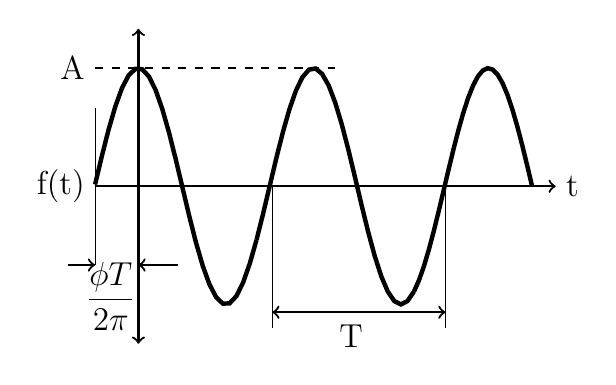
\begin{tikzpicture}
\draw[thick,<->] (0,-2)--(0,2); %yaxis
\draw[thick,->](-.55,0)--(5.3,0); %xaxis
\draw (-.55,1)--(-.55,-1);
\draw (1.7,0)--(1.7,-1.8);
\draw(3.9,0)--(3.9,-1.8);
\draw[thick,<->](1.7,-1.6)--(3.9,-1.6);
\draw[thick,->](-.9,-1)--(-.55,-1);
\draw[thick,<-](0,-1)--(.5,-1);
\node[right,thick,font=\large] at(5.3,0){t};
\draw[dashed, thick](-.55,1.5)--(2.5,1.5); %amplitude
\node[thick,left,font=\large] at (-.55,1.5){A}; %amplitude label
\node[thick,left,font=\large] at (-.55,0){f(t)}; %f(t) label
\node[thick,font=\large] at (2.7,-1.9){T}; %T label
\node[thick,font=\large] at (-.35,-1.4){$\dfrac{\phi T}{2\pi}$}; %phase label

\draw[ultra thick,domain=-.55:1.5] plot (\x,{1.5*cos(\x*162)}); %sine
\draw[ultra thick,domain=1.5:3.5] plot (\x,{1.5*cos(\x*162)}); %sine
\draw[ultra thick,domain=3.5:5] plot (\x,{1.5*cos(\x*162)}); %sine


%\node[thick] at (15.3,0) {0 $V$}; %0 Volts label
%\draw[thick,<->](1.05,1)--(1.05,3); %V_p
%\node[black,fill=white,draw=white,shape=rectangle,scale=1] at (1.05,2.1) {$V_p$}; %V_p label
\end{tikzpicture}

\caption{Phase shifting of a sine wave.}
\label{fig:fs1}
\end{marginfigure}

The quantity 2$\pi$/T=2$\pi$f is known as the {\bf angular frequency}.

Sine waves are added together to form Fourier series. In this light, the addition properties of two sine waves is a special case of Fourier series. If the frequency and the phase are identical, then the amplitude of the sum is the sum of the amplitudes. The frequency and phase remain unchanged. This means that

\begin{equation}
A\sin\left( \dfrac{2\pi}{T}t+\theta \right)+B\sin\left(\dfrac{2\pi}{T}t+\theta\right)=\sin\left(\dfrac{2\pi}{T}t+\theta\right)
\label{equ:fs2}
\end{equation}

The addition of sines with the same frequency but {\bf different} phases introduces new properties. Suppose the two signals are separated by a phase of $\pi$/2. Then

\begin{equation}
A\sin\left(\dfrac{2\pi}{T}t\right)+B\sin\left(\dfrac{2\pi}{T}t+\dfrac{\pi}{2}\right)=C\sin\left(\dfrac{2\pi}{T}t+\phi\right)
\label{equ:fs3}
\end{equation}

where

\begin{equation}
C=\sqrt{A^2+B^2}
\label{equ:fs4}
\end{equation}

and

\begin{equation}
\phi=\tan^{-1}\left(\dfrac{B}{A}\right)
\label{equ:fs5}
\end{equation}

The amplitude and phase of the sum are now {\bf functions} of the amplitude and phase of the addends and are given by Equations \ref{equ:fs4} and \ref{equ:fs5}. However, the frequency remains unchanged and the sum is still a sine wave. 

When sine waves of different frequencies are added, the sum is no longer a sine wave. For example, if sines of identical amplitude and unequal but close frequency are added, the result takes the form shown in Figure \ref{fig:fs2}. This is the phenomenon known as {\bf beats}. A lower frequency envelope is seen to be riding on the outside of a higher frequency signal, known as a {\bf carrier}, because it "carries" the lower frequency beat signal along.

\begin{marginfigure}
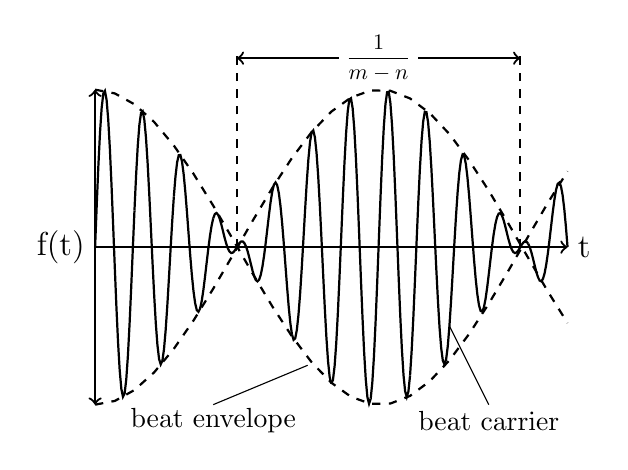
\begin{tikzpicture}

\draw[thick,<->] (0,-2)--(0,2); %yaxis
\draw[thick,->](0,0)--(6,0); %xaxis
\node[thick,left,font=\large] at (0,0){f(t)};
\draw[thick,dashed](1.8,0)--(1.8,2.5);
\draw[thick,dashed](5.4,0)--(5.4,2.5);
\draw[thick,<->](1.8,2.4)--(5.4,2.4);
\node[black,fill=white,shape=rectangle,scale=.8]at (3.6,2.4){$\dfrac{1}{m-n}$}; %beat freq
\node[thick] at (1.5,-2.2){beat envelope}; %envelope label
\node[thick] at (5,-2.2){beat carrier}; %carrier label
\node[thick,right,font=\large] at (6,0){t};
\draw(1.5,-2)--(2.7,-1.5);
\draw(5,-2)--(4.5,-1);

\draw[thick,domain=0:.5] plot (\x,{sin(\x*800)+sin(\x*700)}); %carrier
\draw[thick,domain=.5:1] plot (\x,{sin(\x*800)+sin(\x*700)}); %carrier
\draw[thick,domain=1:1.5] plot (\x,{sin(\x*800)+sin(\x*700)}); %carrier
\draw[thick,domain=1.5:2] plot (\x,{sin(\x*800)+sin(\x*700)}); %carrier
\draw[thick,domain=2:2.5] plot (\x,{sin(\x*800)+sin(\x*700)}); %carrier
\draw[thick,domain=2.5:3] plot (\x,{sin(\x*800)+sin(\x*700)}); %carrier
\draw[thick,domain=3:3.5] plot (\x,{sin(\x*800)+sin(\x*700)}); %carrier
\draw[thick,domain=3.5:4] plot (\x,{sin(\x*800)+sin(\x*700)}); %carrier
\draw[thick,domain=4:4.5] plot (\x,{sin(\x*800)+sin(\x*700)}); %carrier
\draw[thick,domain=4.5:5] plot (\x,{sin(\x*800)+sin(\x*700)}); %carrier
\draw[thick,domain=5:5.5] plot (\x,{sin(\x*800)+sin(\x*700)}); %carrier
\draw[thick,domain=5.5:6] plot (\x,{sin(\x*800)+sin(\x*700)}); %carrier

\draw[thick,domain=0:6,dashed] plot (\x,{2*cos(\x*49.8)}); %envelope
\draw[thick,domain=0:6,dashed] plot (\x,{-2*cos(\x*49.8)}); %envelope
\end{tikzpicture}
\caption{An illustration of beat frequency.}
\label{fig:fs2}
\end{marginfigure}

Mathematically, adding a sine wave of frequency n to a sine wave of frequency m yields the expression

\begin{equation}
sin(nx)+sin(mx)=2sin\left[2\pi\left(\dfrac{m+n}{2}\right)x\right]cos\left[2\pi\left(\dfrac{m-n}{2}\right)x\right]
\label{equ:fs6}
\end{equation}

If $m$ and $n$ are close together, then Equation \ref{equ:fs6} can be thought of as a time varying amplitude applied to a sine wave of frequency $(m+n)/2$. Although this time varying amplitude has frequency $(m-n)/2$, Figure \ref{fig:fs2} shows that the frequency at which the minimum value appears is {\bf twice} this amount. So the beat envelope is heard as the $m-n$.

The results of Equations \ref{equ:fs2} through \ref{equ:fs6} are found by use of standard trigonometric identities and result in waves that are repetitive in nature. However, the resulting sum of two sine waves {\bf need not repeat itself}. An interesting fact about the addition of different frequencies, $m$ and $n$, is that the resulting wave is periodic only if $m$ and $n$ are {\bf commensurable}. Two numbers $m$ and $n$ are commensurable if there exists two rational numbers $p$ and $q$ such that

\begin{equation}
pm=qn
\label{equ:fs7}
\end{equation}

If the frequencies $m$ and $n$ are commensurable, then the frequency of the sum is given by the {\bf greatest common divisor} of $m$ and $n$.

A Fourier series generalizes the sum of two sine waves to the sum of an arbitrary number of sine and cosine waves. Each element of the series can have a different amplitude. However, the frequency of any element must be an integer multiple of one frequency known as the {\bf fundamental}. The integer multiples of the fundamental are known as {\bf harmonics}. Suppose the fundamental has a period $T$. Then a Fourier series has the form 

\begin{equation}
f(t)=a_0+\sum^{\infty}_{n=1}\left(a_ncos\left(\dfrac{2nt\pi}{T}\right)+b_nsin\left(\dfrac{2nt\pi}{T}\right)\right)
\label{equ:fs8}
\end{equation}

The constants $a_0$, $a_1$, $a_2$... $b_1$, $b_2$... are called {\bf Fourier coefficients}. The most significant property of Fourier series is that {\bf any} function, $f(t)$, that repeats with a period T can be represented by such a series. This includes waves with sudden jumps and sharp corners.

A crucial problem is how to find the Fourier coefficients $a_0$, $a_n$ and $b_n$ for a given function $f(t)$. What Fourier found was a method for determining these coefficients. The Fourier coefficients are calculated by the formulae

\begin{equation}
a_0=\dfrac{1}{T}\int_0^Tf(t)dt
\label{equ:fs9}
\end{equation}

\begin{equation}
a_n=\dfrac{2}{T}\int_0^Tf(t)cos\left(\dfrac{2n\pi}{T}t\right)dt
\label{equ:fs10}
\end{equation}

and

\begin{equation}
b_n=\dfrac{2}{T}\int_0^Tf(t)sin\left(\dfrac{2n\pi}{T}t\right)dt
\label{equ:fs11}
\end{equation}

It can be seen from Equations \ref{equ:fs9}, \ref{equ:fs10}, and \ref{equ:fs11} that the Fourier coefficients for a function f(t) are found by some form of integration over the period $T$. The reason for this is that certain integrals have the useful property of being zero for all terms of the Fourier series {\bf except one}. They act as a {\bf filter} that preserves one term of the Fourier series and eliminates all the others.

Equation \ref{equ:fs9} suggests that integrating the function and dividing by the period yields $a_o$. Since $f(t)$ has a Fourier series, integrating $f(t)$ gives

\footnotesize
\begin{equation}
\int_0^Tf(t)=\int_0^T\left[a_0+a_1\cos\left(\dfrac{2\pi}{T}t\right)+a_2\cos\left(\dfrac{4\pi}{T}t\right)+...b_1\sin\left(\dfrac{2\pi}{T}t\right)+...\right]dt
\label{equ:fs12}
\end{equation}
\normalsize

Another useful property of integrals is that each element of a sum can be integrated separately. So,

\small
\begin{multline}
\int_0^Tf(t)=\int_0^Ta_0dt+\int_0^Ta_1cos\left(\dfrac{2\pi}{T}t\right)dt
+\int_0^Ta_2\cos\left(\dfrac{4\pi}{T}t\right)dt\\+...\int_0^Tb_1\sin\left(\dfrac{2\pi}{T}t\right)dt+...
\label{equ:fs13}
\end{multline}
\normalsize

However, the net area under a full period of any sine or cosine is zero, so all the integrals on the right {\bf vanish} except for $a_o$. This gives

\begin{equation}
\int_0^Tf(t)dt=\int_0^Ta_0dt=Ta_0
\label{equ:fs14}
\end{equation}

Therefore, $a_o$, the first Fourier coefficient, is found to be Equation \ref{equ:fs9}.

The procedure for deducing $a_n$ is nearly identical. Two additional integral properties are needed as filters. It turns out that the integral over a full period of $sin(mx)cos(nx)$ is always zero. Also, the integral over a full period of $cos(mx)cos(nx)$ is always zero {\bf except} when $m=n$. This filters out all the $a_n$ terms but one.

Using these facts, it can be seen that

\begin{equation}
\int_0^Tf(t)\cos\left(\dfrac{2n\pi}{T}t\right)dt=\int_0^Ta_n\cos^2\left(\dfrac{2n\pi}{T}t\right)dt
\label{equ:fs15}
\end{equation}

This reduces to

\begin{equation}
\int_0^Tf(t)\cos\left(\dfrac{2n\pi}{T}t\right)dt=\dfrac{a_nT}{2}
\label{equ:fs16}
\end{equation}

which gives Equation \ref{equ:fs10}.

The determination of $b_n$ is identical except for the filtering property needed to isolate one $b_n$ term. The integral over a full period of $sin(mx)sin(nx)$ as always zero except when $m=n$. This gives

\begin{equation}
\int_0^Tf(t)\sin\left(\dfrac{2n\pi}{T}t\right)dt=\dfrac{b_nT}{2}
\label{equ:fs17}
\end{equation}

Thus, for a given periodic function, f(t), Equations \ref{equ:fs9}, \ref{equ:fs10} and \ref{equ:fs11} can be used to find the Fourier coefficients. Once these are known, the Fourier series can be used to represent or approximate $f(t)$. For example, Figure \ref{fig:fs3} shows a square wave. This signal is not smooth at all. Nevertheless, it has a Fourier series. It turns out that for this square wave $a_0=0$, $a_n=0$ and $b_n=0$ if $n$ is even and $b_n=1/n$ if $n$ is odd. This implies that a square wave is composed of a fundamental sine wave and all of the odd harmonics. Figure \ref{fig:fs3} shows two other signals superimposed on the square wave. One signal is the fundamental, corresponding to the coefficient $b_1$. The other curve is the sum of the first four odd harmonics and the fundamental, namely, $b_1$, $b_3$, $b_5$, $b_7$, and $b_9$.

\begin{figure}

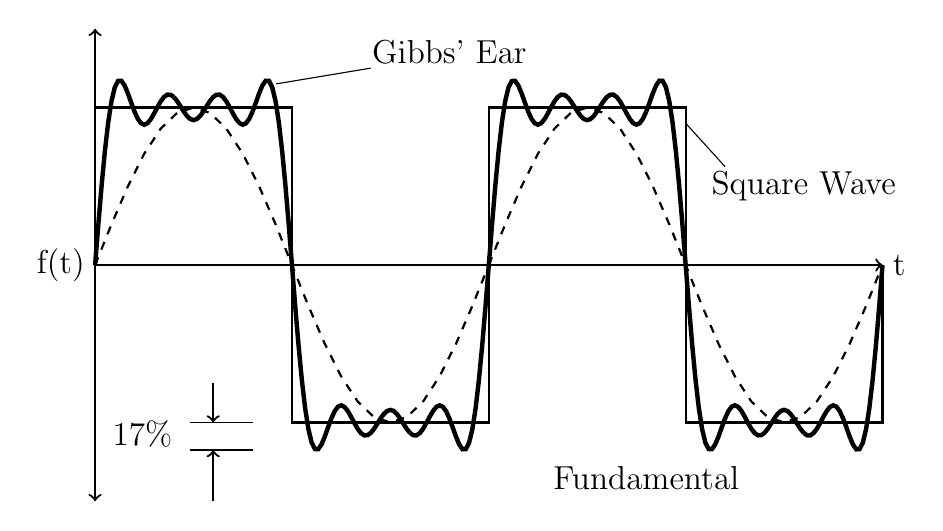
\begin{tikzpicture}

\draw[thick,<->] (0,-3)--(0,3); %yaxis
\draw[thick,->](0,0)--(10,0); %xaxis

%some labels
\node[thick,left,font=\large] at (0,0){f(t)};
\node[thick,right,font=\large] at (10,0){t};
\node[thick,font=\large] at (4.5,2.7){Gibbs' Ear};
\node[thick,font=\large] at (9,1){Square Wave};
\node[thick,font=\large] at (7,-2.7){Fundamental};
\node[thick,font=\large] at (.6,-2.15){17\%};

%some lines
\draw[thick,->] (1.5,-3)--(1.5,-2.35);
\draw[thick,->] (1.5,-1.5)--(1.5,-2);
\draw(1.2,-2)--(2,-2);
\draw(1.2,-2.35)--(2,-2.35);
\draw(3.5,2.5)--(2.3,2.3);
\draw(8,1.25)--(7.5,1.8);

%some functions
\draw[thick,domain=0:5,dashed] plot (\x, {2*sin(\x*72)}); %first order FS
\draw[thick,domain=5:10,dashed] plot (\x, {2*sin(\x*72)}); %first order FS
\draw[thick](0,2)--(2.5,2)--(2.5,-2)--(5,-2)--(5,2)--(7.5,2)--
(7.5,-2)--(10,-2)--(10,0); %square wave

%4th order FS
\draw[ultra thick,domain=0:1] plot (\x, {2*(1.27*sin(\x*1.2566 r)+.42*sin(\x*3.7699 r)+.25*sin(\x*6.2832 r)
+.18*sin(\x*8.7965 r))});
\draw[ultra thick,domain=1:2] plot (\x, {2*(1.27*sin(\x*1.2566 r)+.42*sin(\x*3.7699 r)+.25*sin(\x*6.2832 r)
+.18*sin(\x*8.7965 r))});
\draw[ultra thick,domain=2:3] plot (\x, {2*(1.27*sin(\x*1.2566 r)+.42*sin(\x*3.7699 r)+.25*sin(\x*6.2832 r)
+.18*sin(\x*8.7965 r))});
\draw[ultra thick,domain=3:4] plot (\x, {2*(1.27*sin(\x*1.2566 r)+.42*sin(\x*3.7699 r)+.25*sin(\x*6.2832 r)
+.18*sin(\x*8.7965 r))});
\draw[ultra thick,domain=4:5] plot (\x, {2*(1.27*sin(\x*1.2566 r)+.42*sin(\x*3.7699 r)+.25*sin(\x*6.2832 r)
+.18*sin(\x*8.7965 r))});
\draw[ultra thick,domain=5:6] plot (\x, {2*(1.27*sin(\x*1.2566 r)+.42*sin(\x*3.7699 r)+.25*sin(\x*6.2832 r)
+.18*sin(\x*8.7965 r))});
\draw[ultra thick,domain=6:7] plot (\x, {2*(1.27*sin(\x*1.2566 r)+.42*sin(\x*3.7699 r)+.25*sin(\x*6.2832 r)
+.18*sin(\x*8.7965 r))});
\draw[ultra thick,domain=7:8] plot (\x, {2*(1.27*sin(\x*1.2566 r)+.42*sin(\x*3.7699 r)+.25*sin(\x*6.2832 r)
+.18*sin(\x*8.7965 r))});
\draw[ultra thick,domain=8:9] plot (\x, {2*(1.27*sin(\x*1.2566 r)+.42*sin(\x*3.7699 r)+.25*sin(\x*6.2832 r)
+.18*sin(\x*8.7965 r))});
\draw[ultra thick,domain=9:10] plot (\x, {2*(1.27*sin(\x*1.2566 r)+.42*sin(\x*3.7699 r)+.25*sin(\x*6.2832 r)
+.18*sin(\x*8.7965 r))});
\end{tikzpicture}

\caption{An illustration of Gibbs' phenomenon.}
\label{fig:fs3}
\end{figure}


It can be seen that the shape is converging to a square wave. However, there seems to be a greater difficulty for the Fourier series to track at the discontinuity. There is a sudden jump or overshoot just before each rise and fall. This propensity for a Fourier series to overshoot at the edges is called {\bf Gibb's phenomenon} or {\bf Gibbs Ears}. It turns out that this behavior is a general property of all Fourier series, not just the square wave. In fact, as more terms are added, the ears get narrower but their height {\bf may not decrease}. For the square wave, it can be shown that the height of the ears never falls below 17\% above the square wave level.

This experiment examines the wave phenomena described here using an instrument called a {\bf Fourier Synthesizer}. A Fourier synthesizer is an instrument that creates arbitrarily shaped periodic signals by use of Fourier series. The device generates two sine waves at a fundamental frequency of 440 Hz, as well as eight other harmonic sine waves at frequencies of 880 Hz, 1320 Hz,... up to 3960 Hz. The phase and amplitude of each of these ten signals can be independently adjusted. Any combination of them can be added together. In this way the synthesizer can generate the first nine terms of any Fourier series.

\begin{figure}
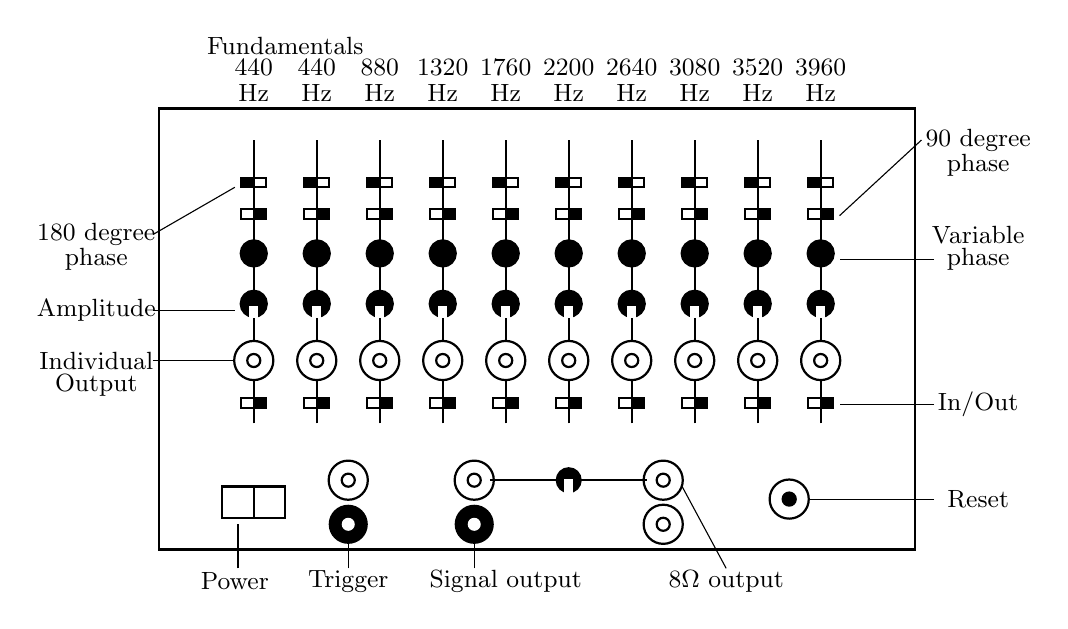
\begin{tikzpicture}[thick,scale=.8,font=\small]
\draw(0,0)rectangle(12,7); %box
\foreach \x in {0,1,2,3,4,5,6,7,8,9}
{
\begin{scope}[shift={(.5,0)}]
%dials
\draw(1+\x,2)--(1+\x,6.5);
\node[black,fill=white,draw=black,shape=circle,scale=1.5] at (1+\x,3){};
\node[black,fill=white,draw=black,shape=circle,scale=.5] at (1+\x,3){};
\draw(.8+\x,2.25)rectangle(1+\x,2.4);
\draw[fill=black](1+\x,2.25)rectangle(1.2+\x,2.4);
\node[black,fill=black,draw=black,shape=circle,scale=1] at (1+\x,3.9){};
\node[black,fill=black,draw=black,shape=circle,scale=1] at (1+\x,4.7){};
\draw(.8+\x,5.25)rectangle(1+\x,5.4);
\draw[fill=black](1+\x,5.25)rectangle(1.2+\x,5.4);
\draw[fill=black](.8+\x,5.75)rectangle(1+\x,5.9);
\draw[fill=white](1+\x,5.75)rectangle(1.2+\x,5.9);
\draw[fill=white,draw=white](.95+\x,3.7)rectangle(1.05+\x,3.85);
\node at (1+\x,7.25){Hz};
\end{scope}
}
\draw(1,.5)rectangle(2,1);
\draw(1.5,.5)--(1.5,1);
\node[fill=black,shape=circle,scale=1.5] at (3,.4){}; %trigger
\node[fill=white,shape=circle,scale=.5] at (3,.4){}; %trigger
\node[draw=black,fill=white,shape=circle,scale=1.5] at (3,1.1){};
\node[draw=black,fill=white,shape=circle,scale=.5] at (3,1.1){};
\node[fill=black,shape=circle,scale=1.5] at (5,.4){}; %signal output
\node[fill=white,shape=circle,scale=.5] at (5,.4){}; %signal output
\node[draw=black,fill=white,shape=circle,scale=1.5] at (5,1.1){}; %8ohm output
\node[draw=black,fill=white,shape=circle,scale=.5] at (5,1.1){}; %8ohm output
\node[draw=black,fill=white,shape=circle,scale=1.5] at (8,1.1){}; %8ohm output
\node[draw=black,fill=white,shape=circle,scale=.5] at (8,1.1){}; %8ohm output
\node[draw=black,fill=white,shape=circle,scale=1.5] at (8,.4){}; %8ohm output
\node[draw=black,fill=white,shape=circle,scale=.5] at (8,.4){}; %8ohm output
\node[draw=black,fill=white,shape=circle,scale=1.5] at (10,.8){}; %reset
\node[draw=black,fill=black,shape=circle,scale=.5] at (10,.8){}; %reset
\draw(5.25,1.1)--(7.75,1.1);
\node[fill=black,shape=circle,scale=1] at (6.5,1.1){};
\draw[fill=white,draw=white](6.45,.9)rectangle(6.55,1.1);
%labels
\node at (2,8){Fundamentals};
\node at (1.5,7.65){440};
\node at (2.5,7.65){440};
\node at (3.5,7.65){880};
\node at (4.5,7.65){1320};
\node at (5.5,7.65){1760};
\node at (6.5,7.65){2200};
\node at (7.5,7.65){2640};
\node at (8.5,7.65){3080};
\node at (9.5,7.65){3520};
\node at (10.5,7.65){3960};
\node at (-1,5){180 degree};
\node at (-1,4.6){phase};
\draw[thin](-.1,5)--(1.2,5.75);
\node at (-1,3.8){Amplitude};
\draw[thin](-.1,3.8)--(1.2,3.8);
\node at (-1,3){Individual};
\node at (-1,2.6){Output};
\draw[thin](-.1,3)--(1.2,3);
\node at (13,6.5){90 degree};
\node at (13,6.1){phase};
\draw[thin](12.1,6.5)--(10.8,5.3);
\node at (13,5){Variable};
\node at (13,4.6){phase};
\draw[thin](12.3,4.6)--(10.8,4.6);
\node at (13,2.3){In/Out};
\draw[thin](12.3,2.3)--(10.8,2.3);
\node at (13,.8){Reset};
\draw[thin](12.3,.8)--(10.3,.8);
\node at (9,-.5){8$\Omega$ output};
\draw[thin](9,-.3)--(8.3,1);
\node at (5.5,-.5){Signal output};
\draw[thin](5,-.3)--(5,.1);
\node at (3,-.5){Trigger};
\draw[thin](3,-.3)--(3,.1);
\node at (1.2,-.5){Power};
\draw[thin](1.25,-.3)--(1.25,.4);
\end{tikzpicture}
\caption{A Fourier synthesizer.}
\label{fig:fs4}
\end{figure}

The Fourier synthesizer used in this experiment is shown in Figure \ref{fig:fs4}. There are ten columns of controls. One column for each of the two fundamentals and eight harmonics. At the top of each column are the phase controls. Two switches select 90$^{\circ}$ and 180$^{\circ}$ phase shifts. The third phase control is continuously variable over a 90$^{\circ}$ range. Together, these three controls provide a full 360$^{\circ}$ phase adjustment range. Below the phase controls is an amplitude control to set the size of the signal. An in/out switch selects whether the column gets added to the output or not. Each column also includes an output point where the signal generated by that column can be measured.

The three primary signal outputs generated by the synthesizer lie below the ten columns. All of the selected columns (those that are switched in) are {\bf added} together and presented at the 10 k$\Omega$ output and the 8 $\Omega$ output. The 10 k$\Omega$ output is connected to an oscilloscope for viewing and measurement of the generated signal  The 8 $\Omega$ output is used to drive a speaker for audible output.

The third output is called a {\bf trigger}. This signal is a square wave locked in phase with the fundamental. The edges of this square wave represent a phase angle of 0$^{\circ}$. This signal serves as a time marker (metronome) against which phases can be measured. Lastly, the reset button is used to periodically resynchronize all the harmonics back together.

The synthesizer can be used to experimentally examine the properties of the addition of sine waves. Equation \ref{equ:fs3} can be examined by adding a sine wave to another phase shifted sine wave of the identical frequency. The amplitude and phase of the sum would be expected to vary in the systematic manner suggested by Equations \ref{equ:fs4} and \ref{equ:fs5}. 

Equation \ref{equ:fs6} and Figure \ref{fig:fs2} can be tested by observing the resulting waveform when sines of identical amplitude but differing frequency are added together. For best results, the chosen frequencies should be relatively close together. This suggests adding together high harmonics such as 5, 6, 7, 8 and 9. The resulting frequencies of the beat envelope and the beat carrier can be measured with an oscilloscope and compared against Equation \ref{equ:fs6}.

Similarly, Equation \ref{equ:fs7} can be examined by adding together two sinusoids of arbitrary amplitude, phase and frequency. The sum would be expected to have a frequency given by the greatest common divisor, independent of the amplitude and phase. 

Most importantly, Equations \ref{equ:fs9}, \ref{equ:fs10} and \ref{equ:fs11} can be used to find Fourier coefficients for various signals. The coefficients for a wide variety of common signals have been precomputed for implementation on the synthesizer. The selected signals are chosen from a variety of areas of electrical engineering and physics. It should be noted that the resulting shape is quite sensitive to the actual amplitude and phase of each harmonic. For best results, the amplitude of each harmonic should be set using the multimeter and the phase should be set using the oscilloscope.

\section{Experimental Procedure}
\begin{enumerate}
\item Connect the Fourier synthesizer to the oscilloscope. One channel on the oscilloscope is best left connected to the trigger. The second channel on the oscilloscope is used to view the signal output or the individual output of each harmonic, whichever is most useful. The multimeter is connected to the individual output of whichever wave needs to be measured at the time. A common ground should be used between all the equipment. For best results, the oscilloscope should be  AC coupled.


\begin{marginfigure}
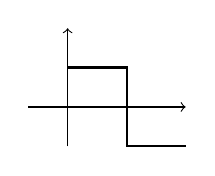
\begin{tikzpicture}
\draw[->](0,-.5)--(0,1);
\draw[->](-.5,0)--(1.5,0);
\draw[thick](0,.5)--(.75,.5)--(.75,-.5)--(1.5,-.5);
\end{tikzpicture}
\caption*{Square Wave}
\label{fig:fs5}
\end{marginfigure}

\begin{marginfigure}
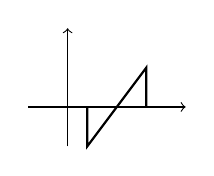
\begin{tikzpicture}
\draw[->](0,-.5)--(0,1);
\draw[->](-.5,0)--(1.5,0);
\draw[thick](.25,0)--(.25,-.5)--(1,.5)--(1,0);
\end{tikzpicture}
\caption*{Ramp Function}
\label{fig:fs6}
\end{marginfigure}

\begin{marginfigure}
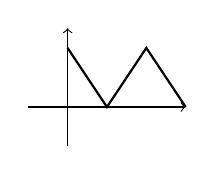
\begin{tikzpicture}
\draw[->](0,-.5)--(0,1);
\draw[->](-.5,0)--(1.5,0);
\draw[thick](0,.75)--(.5,0)--(1,.75)--(1.5,0);
\end{tikzpicture}
\caption*{Triangle Wave}
\label{fig:fs7}
\end{marginfigure}

\begin{marginfigure}
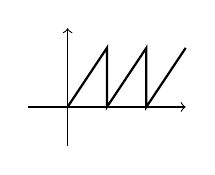
\begin{tikzpicture}
\draw[->](0,-.5)--(0,1);
\draw[->](-.5,0)--(1.5,0);
\draw[thick](0,0)--(.5,.75)--(.5,0)--(1,.75)--(1,0)--(1.5,.75);
\end{tikzpicture}
\caption*{Sawtooth Wave}
\label{fig:fs8}
\end{marginfigure}

\begin{marginfigure}
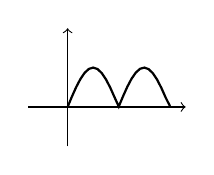
\begin{tikzpicture}
%\draw[<->](0,1)--(0,0)--(1.5,0);
\draw[->](0,-.5)--(0,1);
\draw[->](-.5,0)--(1.5,0);
\draw[thick,domain=0:1.3] plot (\x, {.5*abs(sin(\x*278))});
\end{tikzpicture}
\caption*{Full Wave}
\label{fig:fs9}
\end{marginfigure}

\begin{marginfigure}
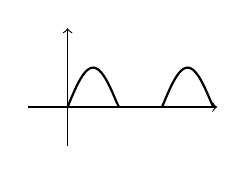
\begin{tikzpicture}
%\draw[<->](0,1)--(0,0)--(1.9,0);
\draw[->](0,-.5)--(0,1);
\draw[->](-.5,0)--(1.9,0);
\draw[thick,domain=0:.65] plot (\x, {.5*abs(sin(\x*278))});
\draw[thick](.65,0)--(1.2,0);
\draw[thick,domain=1.2:1.85] plot (\x, {.5*abs(sin((\x-1.2)*278))});
\end{tikzpicture}
\caption*{Half Wave}
\label{fig:fs10}
\end{marginfigure}



\item To test Equation \ref{equ:fs3}, choose one fundamental to have an amplitude A and the other amplitude B. Set the phase of A to be 0$^{\circ}$ and the phase of B to be 90$^{\circ}$. The phase is set using the oscilloscope, by observing the alignment of the sine wave against one edge of the trigger. A phase shift of 90$^{\circ}$ is 90$^{\circ}$/360$^{\circ}$=1/4 of a period. Since the period is 1/440 s, the time shift for 90$^{\circ}$ is $0.25/440570$ s$\approx 570$ $\mu s$. Fix the amplitude of A to some known value using the multimeter. Then, for at least eight different amplitudes of B, measure the amplitude of and phase of the sum. Amplitude is best measured with the AC voltmeter, and phase is best measured with the oscilloscope.

\item Choose any {\bf one} of the following tests for the addition of sine waves of different frequency.

\begin{enumerate}[label=(\Alph*)]
\item Examine beats as given by Equation \ref{equ:fs6} and Figure \ref{fig:fs2}. Choose any two neighboring higher harmonics and set their amplitudes to be equal and the phases to be 0$^{\circ}$. Measure the frequency of the beat envelope and beat carrier. Repeat for at least two other neighboring harmonics.

\item Examine the sum frequency predicted by Equation \ref{equ:fs7}. Choose any two frequencies with arbitrary non zero amplitudes and arbitrary phase. Measure the period of their sum. The sum frequency can be compared to the expected value given by the greatest common divisor of the individual frequencies. Repeat for at least two other combinations.
\end{enumerate}

\item The synthesizer can generate a 9 term Fourier series for the square wave, as seen in Figure \ref{fig:fs3}. A recipe for synthesizing the square is given in Table \ref{tab:fs1}. To synthesize a particular wave shape, each harmonic 1 through 9 must be set to a particular amplitude and phase. Each amplitude in the table is a percentage relative to a maximum amplitude within the first nine terms. Each phase angle is the number of degrees by which to shift that harmonic. Again, for best results, the AC voltmeter should be used to set the amplitude and the oscilloscope used to set the phase. Synthesize the square wave.

\begin{table}[h]
\small
\begin{tabular}{c|c|c|c|c|c|c|c|c|c|c|}
\cline{2-11}
&n&1&2&3&4&5&6&7&8&9\\ \hline
\multicolumn{1}{|c|}{\multirow{2}{*}{Square}}&\% Ampl.&100&0.0&33.3&0.0&20.0&0.0&14.3&0.0&11.1\\
\multicolumn{1}{|c|}{}&Phase&90$^{\circ}$&0$^{\circ}$&90$^{\circ}$&0$^{\circ}$&90$^{\circ}$&0$^{\circ}$&90$^{\circ}$&0$^{\circ}$&90$^{\circ}$\\ \hline
\end{tabular}
\normalsize

%\stepcounter{figure}
%\smallskip\noindent {Table 1}
\caption{ }
\label{tab:fs1}
\end{table}





\item Gibbs Ears. Gibbs ears can be measured once the square wave has been synthesized. As each harmonic above number 1 is "switched in" record the height and width of Gibb's ears. This data can be used to check whether the width steadily decreases, while the height goes no lower than 17\%.

\item The following signals are commonly found in sweep circuits, used in radar or television. Synthesize any {\bf one} of the following waveforms. Record the result and note where it is different from the ideal shape. When synthesizing your signal {\bf do not} trust the amplitude dials on the synthesizer. Instead set the amplitudes individually by measuring them with a multimeter.


\begin{table}[h]
\scriptsize
\begin{tabular}{c|c|c|c|c|c|c|c|c|c|c|}
\cline{2-11}
&n&1&2&3&4&5&6&7&8&9\\ \hline
\multicolumn{1}{|c|}{\multirow{2}{*}{Ramp}}&\% Ampl.&100&78.5&11.1&39.3&4.0&26.2&2.0&19.6&1.2\\
\multicolumn{1}{|c|}{}&Phase&0$^{\circ}$&270$^{\circ}$&0$^{\circ}$&270$^{\circ}$&0$^{\circ}$&270$^{\circ}$&0$^{\circ}$&270$^{\circ}$&0$^{\circ}$\\ \hline
\multicolumn{1}{|c|}{\multirow{2}{*}{Triangle}}&\% Ampl.&100&0&11.1&0&4.0&0&2.0&0&1.2\\
\multicolumn{1}{|c|}{}&Phase&0$^{\circ}$&0$^{\circ}$&0$^{\circ}$&0$^{\circ}$&0$^{\circ}$&0$^{\circ}$&0$^{\circ}$&0$^{\circ}$&0$^{\circ}$\\ \hline
\multicolumn{1}{|c|}{\multirow{2}{*}{Sawtooth}}&\% Ampl.&100&50&33.3&25.0&20.0&16.7&14.3&12.5&11.1\\
\multicolumn{1}{|c|}{}&Phase&90$^{\circ}$&90$^{\circ}$&90$^{\circ}$&90$^{\circ}$&90$^{\circ}$&90$^{\circ}$&90$^{\circ}$&90$^{\circ}$&90$^{\circ}$\\ \hline
\end{tabular}
\normalsize

%\stepcounter{figure}
%\smallskip\noindent Table 2}
\caption{ }
\label{tab:fs2}
\end{table}


\item The following are signals commonly found in electrical equipment like motors, generators, and power supplies. They are called {\bf rectified sine waves}. Synthesize any one of the following waves. Record the result and note where there is deviation from the ideal desired shape.


\begin{table}[h]
\small
\begin{tabular}{c|c|c|c|c|c|c|c|c|c|c|}
\cline{2-11}
&n&1&2&3&4&5&6&7&8&9\\ \hline
\multicolumn{1}{|c|}{\multirow{2}{*}{Full}}&\% Ampl.&0&100&0&20.0&0&8.6&0&4.8&0\\
\multicolumn{1}{|c|}{}&Phase&0$^{\circ}$&180$^{\circ}$&0$^{\circ}$&180$^{\circ}$&0$^{\circ}$&180$^{\circ}$&0$^{\circ}$&180$^{\circ}$&0$^{\circ}$\\ \hline
\multicolumn{1}{|l|}{\multirow{2}{*}{Half}}&\multicolumn{1}{l|}{\% Ampl.}&\multicolumn{1}{l|}{100}&\multicolumn{1}{l|}{42.4}&\multicolumn{1}{l|}{0}&\multicolumn{1}{l|}{8.5}&\multicolumn{1}{l|}{0}&\multicolumn{1}{l|}{3.6}&\multicolumn{1}{l|}{0}&\multicolumn{1}{l|}{2.0}&\multicolumn{1}{l|}{0}\\
\multicolumn{1}{|l|}{}&\multicolumn{1}{l|}{Phase}&\multicolumn{1}{l|}{90$^{\circ}$}&\multicolumn{1}{l|}{180$^{\circ}$}&\multicolumn{1}{l|}{0$^{\circ}$}&\multicolumn{1}{l|}{180$^{\circ}$}&\multicolumn{1}{l|}{0$^{\circ}$}&\multicolumn{1}{l|}{180$^{\circ}$}&\multicolumn{1}{l|}{0$^{\circ}$}&\multicolumn{1}{l|}{180$^{\circ}$}&\multicolumn{1}{l|}{0$^{\circ}$}\\ \hline
\end{tabular}
\normalsize

%\stepcounter{figure}
%\smallskip\noindent Table 3}
\caption{ }
\label{tab:fs3}
\end{table}

\begin{marginfigure}[+1in]
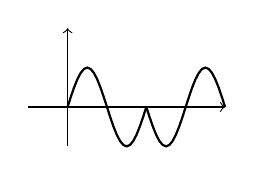
\begin{tikzpicture}
\draw[->](0,-.5)--(0,1);
\draw[->](-.5,0)--(2,0);
\draw[thick,domain=0:1] plot (\x, {.5*sin(\x*360)});
\draw[thick,domain=1:2] plot (\x, {-.5*sin(\x*360)});
\end{tikzpicture}
\caption*{Pulse Shift Keying}
\label{fig:fs11}
\end{marginfigure}

\begin{marginfigure}[+0in]
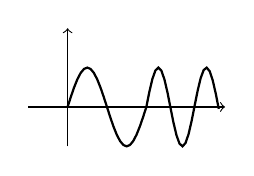
\begin{tikzpicture}
\draw[->](0,-.5)--(0,1);
\draw[->](-.5,0)--(2,0);
\draw[thick,domain=0:1] plot (\x, {.5*sin(\x*360)});
\draw[thick,domain=1:1.92] plot (\x, {.5*sin((\x-1)*590)});
\end{tikzpicture}
\caption*{Frequency Shift Keying}
\label{fig:fs12}
\end{marginfigure}

\begin{marginfigure}[+0in]
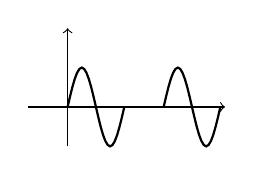
\begin{tikzpicture}
\draw[->](0,-.5)--(0,1);
\draw[->](-.5,0)--(2,0);
\draw(.72,0)--(1.22,0);
\draw[thick,domain=0:.72] plot (\x, {.5*sin(\x*500)});
\draw[thick,domain=1.22:1.94] plot (\x, {.5*sin((\x-.5)*500)});
\end{tikzpicture}
\caption*{Amplitude Shift Keying}
\label{fig:fs13}
\end{marginfigure}




\item Signals of special form are frequently used in digital communication systems. In digital communications there are a number of standard methods for transmitting binary 'ones' and 'zeros.'  Three of these are {\bf Frequency shift keying} (FSK), {\bf amplitude shift keying} (ASK) and {\bf phase shift keying} (PSK). If ASK is used, one cycle of a sine wave represents a 'one' and a flat line is a 'zero.'  Likewise, FSK represents a 'one' by one cycle of a sine wave and represents a 'zero' by one cycle at a different frequency sine wave. For PSK, a 'one' is designated by one cycle of a zero phase and a 'zero' is one cycle of a 180$^{\circ}$ phase shifted sine wave. Generate any {\bf one} of ASK, FSK, or PSK on the synthesizer using the recipes provided. Record the observed shape and note where there is significant deviation from the ideal desired shape.

\begin{table}
\footnotesize
\begin{tabular}{c|c|c|c|c|c|c|c|c|c|c|}
\cline{2-11}
&n&1&2&3&4&5&6&7&8&9\\ \hline
\multicolumn{1}{|c|}{\multirow{2}{*}{PSK}}&\% Ampl.&100&0&60.0&0&14.3&0&6.7&0&3.9\\
\multicolumn{1}{|c|}{}&Phase&0$^{\circ}$&0$^{\circ}$&180$^{\circ}$&0$^{\circ}$&180$^{\circ}$&0$^{\circ}$&180$^{\circ}$&0$^{\circ}$&180$^{\circ}$\\ \hline
\multicolumn{1}{|c|}{\multirow{2}{*}{FSK}}&\% Ampl.&56.8&100.0&41.6&22.0&8.4&0&2.9&2.1&0\\
\multicolumn{1}{|c|}{}&Phase&30$^{\circ}$&150$^{\circ}$&90$^{\circ}$&30$^{\circ}$&330$^{\circ}$&0$^{\circ}$&30$^{\circ}$&330$^{\circ}$&0$^{\circ}$\\ \hline
\multicolumn{1}{|c|}{\multirow{2}{*}{ASK}}&\% Ampl.&84.9&100&50.9&0&12.1&0&5.7&0&3.3\\
\multicolumn{1}{|c|}{}&Phase&0$^{\circ}$&90$^{\circ}$&180$^{\circ}$&0$^{\circ}$&180$^{\circ}$&0$^{\circ}$&180$^{\circ}$&0$^{\circ}$&180$^{\circ}$\\ \hline
\end{tabular}
\normalsize
\caption{ }
\label{tab:fs4}
\end{table}

\newpage
\item The following are {\bf pulse waves} of various {\bf duty cycles}. duty cycle is the proportion of time that the signal is at maximum. Again, generate {\bf one} wave, record it, and note where it diverges from the ideal case. 

\begin{table}
\footnotesize
\begin{tabular}{c|c|c|c|c|c|c|c|c|c|c|}
\cline{2-11}
&n&1&2&3&4&5&6&7&8&9\\ \hline
\multicolumn{1}{|c|}{\multirow{2}{*}{25\%}}&\% Ampl.&100&70.7&33.3&0&20&23.6&14.3&0&11.1\\
\multicolumn{1}{|c|}{}&Phase&45$^{\circ}$&90$^{\circ}$&135$^{\circ}$&0$^{\circ}$&45$^{\circ}$&90$^{\circ}$&135$^{\circ}$&0$^{\circ}$&45$^{\circ}$\\ \hline
\multicolumn{1}{|c|}{\multirow{2}{*}{33\%}}&\% Ampl.&100&50&0&25&20&0&14.3&12.5&0\\
\multicolumn{1}{|c|}{}&Phase&0$^{\circ}$&330$^{\circ}$&0$^{\circ}$&90$^{\circ}$&60$^{\circ}$&0$^{\circ}$&180$^{\circ}$&150$^{\circ}$&0$^{\circ}$\\ \hline
\multicolumn{1}{|c|}{\multirow{2}{*}{8.3\%}}&\% Ampl.&100&95.1&87.3&76.9&64.7&51.3&37.4&23.8&11.1\\
\multicolumn{1}{|c|}{}&Phase&15$^{\circ}$&30$^{\circ}$&45$^{\circ}$&60$^{\circ}$&75$^{\circ}$&90$^{\circ}$&105$^{\circ}$&120$^{\circ}$&180$^{\circ}$\\ \hline
\end{tabular}
\normalsize

%\stepcounter{figure}
%\smallskip\noindent Table 5}
\caption{ }
\label{tab:fs5}
\end{table}

\end{enumerate}


\begin{marginfigure}[+.5in]
\begin{tikzpicture}
\draw[->](0,-.5)--(0,1);
\draw[->](-.5,0)--(2,0);
\draw(0,.75)--(.75,.75)--(.75,-.25)--(2,-.25);
\end{tikzpicture}
\caption*{25\% wave}
\label{fig:fs14}
\end{marginfigure}

\begin{marginfigure}
\begin{tikzpicture}
\draw[->](0,-.5)--(0,1);
\draw[->](-.5,0)--(2,0);
\draw(0,.75)--(.5,.75)--(.5,-.25)--(2,-.25);
\end{tikzpicture}
\caption*{33\% wave}
\label{fig:fs15}
\end{marginfigure}

\begin{marginfigure}
\begin{tikzpicture}
\draw[->](0,-.5)--(0,1);
\draw[->](-.5,0)--(2,0);
\draw(0,.75)--(.25,.75)--(.25,-.25)--(2,-.25);
\end{tikzpicture}
\caption*{8.3\% wave}
\label{fig:fs16}
\end{marginfigure}

\section{Error Analysis}

Generally, the errors in an experiment arise from {\bf systematic errors} in the apparatus and {\bf measurement errors} in the instruments. In this experiment, the measurement errors are determined by the accuracy of the oscilloscope and the multimeter. The systematic errors arise from the behavior and performance of the Fourier synthesizer. The measurement errors of the oscilloscope and multimeter can be readily estimated.

However, there are many possible sources of systematic error lurking inside the synthesizer. The fundamental and harmonic sine waves generated by the synthesizer have some {\bf distortion}. Also, the summation of all the components is not mathematically perfect. Furthermore, the synchronization of the harmonics to each other and to the fundamental is not exact. The magnitude of these and other internal errors is essentially unknown. For this reason error analysis is not required for this experiment.

\section{To be handed in to laboratory instructor.}

%%% begin prelab %%%
\section{PreLab}

Do any {\bf two} of the following three questions.
\begin{enumerate}

\item The synthesizer can generate the first nine terms of a Fourier series. This means that once a1 through to $a_9$ and $b_1$ through to $b_9$ are known for a particular signal, that signal can be synthesized. The n'th term of a Fourier series has the form

\begin{equation}
a_ncos\left(\dfrac{2n\pi}{T}t\right)+b_nsin\left(\dfrac{2n\pi}{T}t\right)
\label{equ:fs18}
\end{equation}

However, the synthesizer does not generate sine and cosine waves. It generates a single wave with adjustable amplitude and phase. Hence, the synthesizer actually generates a Fourier series n'th term of the form

\begin{equation}
A_nsin\left(\dfrac{2n\pi}{T}t+\phi_n\right)
\label{equ:fs19}
\end{equation}

Explain how to find the {\bf amplitude coefficient}, $A_n$, and the {\bf phase coefficient}, $\phi_n$, from the Fourier sine and cosine coefficients $a_n$ and $b_n$.
\item Derive Equation \ref{equ:fs10} or \ref{equ:fs11}.

\item The synthesizer does not generate the $a_0$ term. How does this restrict the types of signals that can be synthesized?  What does AC coupling the oscilloscope have to do with the $a_0$ term?

\end{enumerate}
%%% end prelab %%%

\section{{\bf Data Requirements}}
\begin{enumerate}[resume]

\item A graph of $C^2$ versus $B^2$ from procedure step 2.

\item A graph of tan $\phi$ versus B from procedure step 2.

\item Results and observations from procedure step 3. 

\item A sketch and observations of the synthesized square wave.

\item Data and observations of Gibbs' ears.

\item Sketches and relevant observations for the other synthesized signals.

\section{Discussion}

\item A discussion of the graphs from procedure step 2, the additions of sine waves of equal frequency. Is the synthesizer addition circuitry working correctly?

\item A discussion of the results from the addition of sine waves of different frequency. Is the synthesizer generating harmonic frequencies correctly?

\item Discussion and conclusions for the square wave and Gibb's ears.

\item Conclusions regarding the synthesis of signals by the use of Fourier series.

\end{enumerate}


\AtEndDocument{\clearpage\ifodd\value{page}\else\null\clearpage\fi} % forces even page count, for double siding

\end{document}
